\chapter{Metodología de la Investigación}
\section{Diseño de la investigación}
Según \cite{bk_sampieri2014metodologia} el manipular y encontrar una relación de causa-efecto entre las variables independientes y dependientes son propias de los diseños experimentales.

En el caso de la presente investigación se tiene un diseño experimental porque se pretende establecer la relación entre modelos y técnicas de Deep Learning con el pre-diagnóstico de nódulos tiroideos, esto a través de imágenes de ultrasonido. 

\subsection{Tipo de la investigación}
Ya definido el diseño que tendrá la investigación, se consideró al tipo experimental puro para seguir en la presente investigación, esto ya que la variable independiente (técnicas, modelos y herramientas de Deep Learning) será manipulada constantemente con el fin de encontrar una relación de causalidad ideal con la variable dependiente. Es decir, todo lo relacionado con el Deep Learning será manipulado reiteradas veces con el objetivo de encontrar el impacto en el pre-diagnóstico de nódulos tiroideos. La manipulación en las técnicas o modelos de Deep Learning también incluye a la de la data a usar, ya que se aplicarán diversas técnicas para realizar una limpieza y extracción de características que ayudarán a la posterior elaboración de un algoritmo de diagnóstico asistido.

\subsection{Enfoque de la investigación}
Según \cite{bk_sampieri2014metodologia} el enfoque que sigue una forma secuencial donde no se puede evitar ningún paso, y se usan herramientas estadísticas para realizar mediciones, es el enfoque cuantitativo. 

La presente investigación tiene un enfoque cuantitativo, esto dado que la variable independiente usa valores numéricos y/o estadísticos para su medición. Los resultados de la variable de Deep Learning deberán ser medidos a través de valores numéricos y, en mayor medida, estadísticos.

\subsection{Población}
La población consiste en imágenes de ultrasonido de la glándula de tiroides con presencia de nódulos. Estas imágenes fueron recolectadas de 2421 pacientes por el Zhujiang Hospital of Southem Medical University y debidamente validadas por los comités de ética institucionales en China.

\subsection{Muestra}
La muestra consiste en 3493 imágenes de ultrasonido de la glándula de tiroides recopiladas de 2421 pacientes.

\section{Metodología de Implementación de la Solución}
La metodología por seguir para implementar un modelo de Deep Learning está basado en gran medida en el conocido ciclo de vida de desarrollo de modelos de Inteligencia Artificial, del cual gran parte de los antecedentes mostrados anteriormente siguen con algunas variaciones. 

En el presente caso, se pretende desarrollar un modelo de Deep Learning capaz de brindar ayuda en el diagnóstico médico; por tal motivo, se optó por basar metodología de esta investigación en la de \cite{pr_monroy2021disvc}, modificándolo en cierta medida en el contexto de nódulos tiroideos e imágenes de ultrasonido. A continuación, se presente de forma gráfica la metodología a seguir.

\begin{figure}[H]
	\begin{center}
		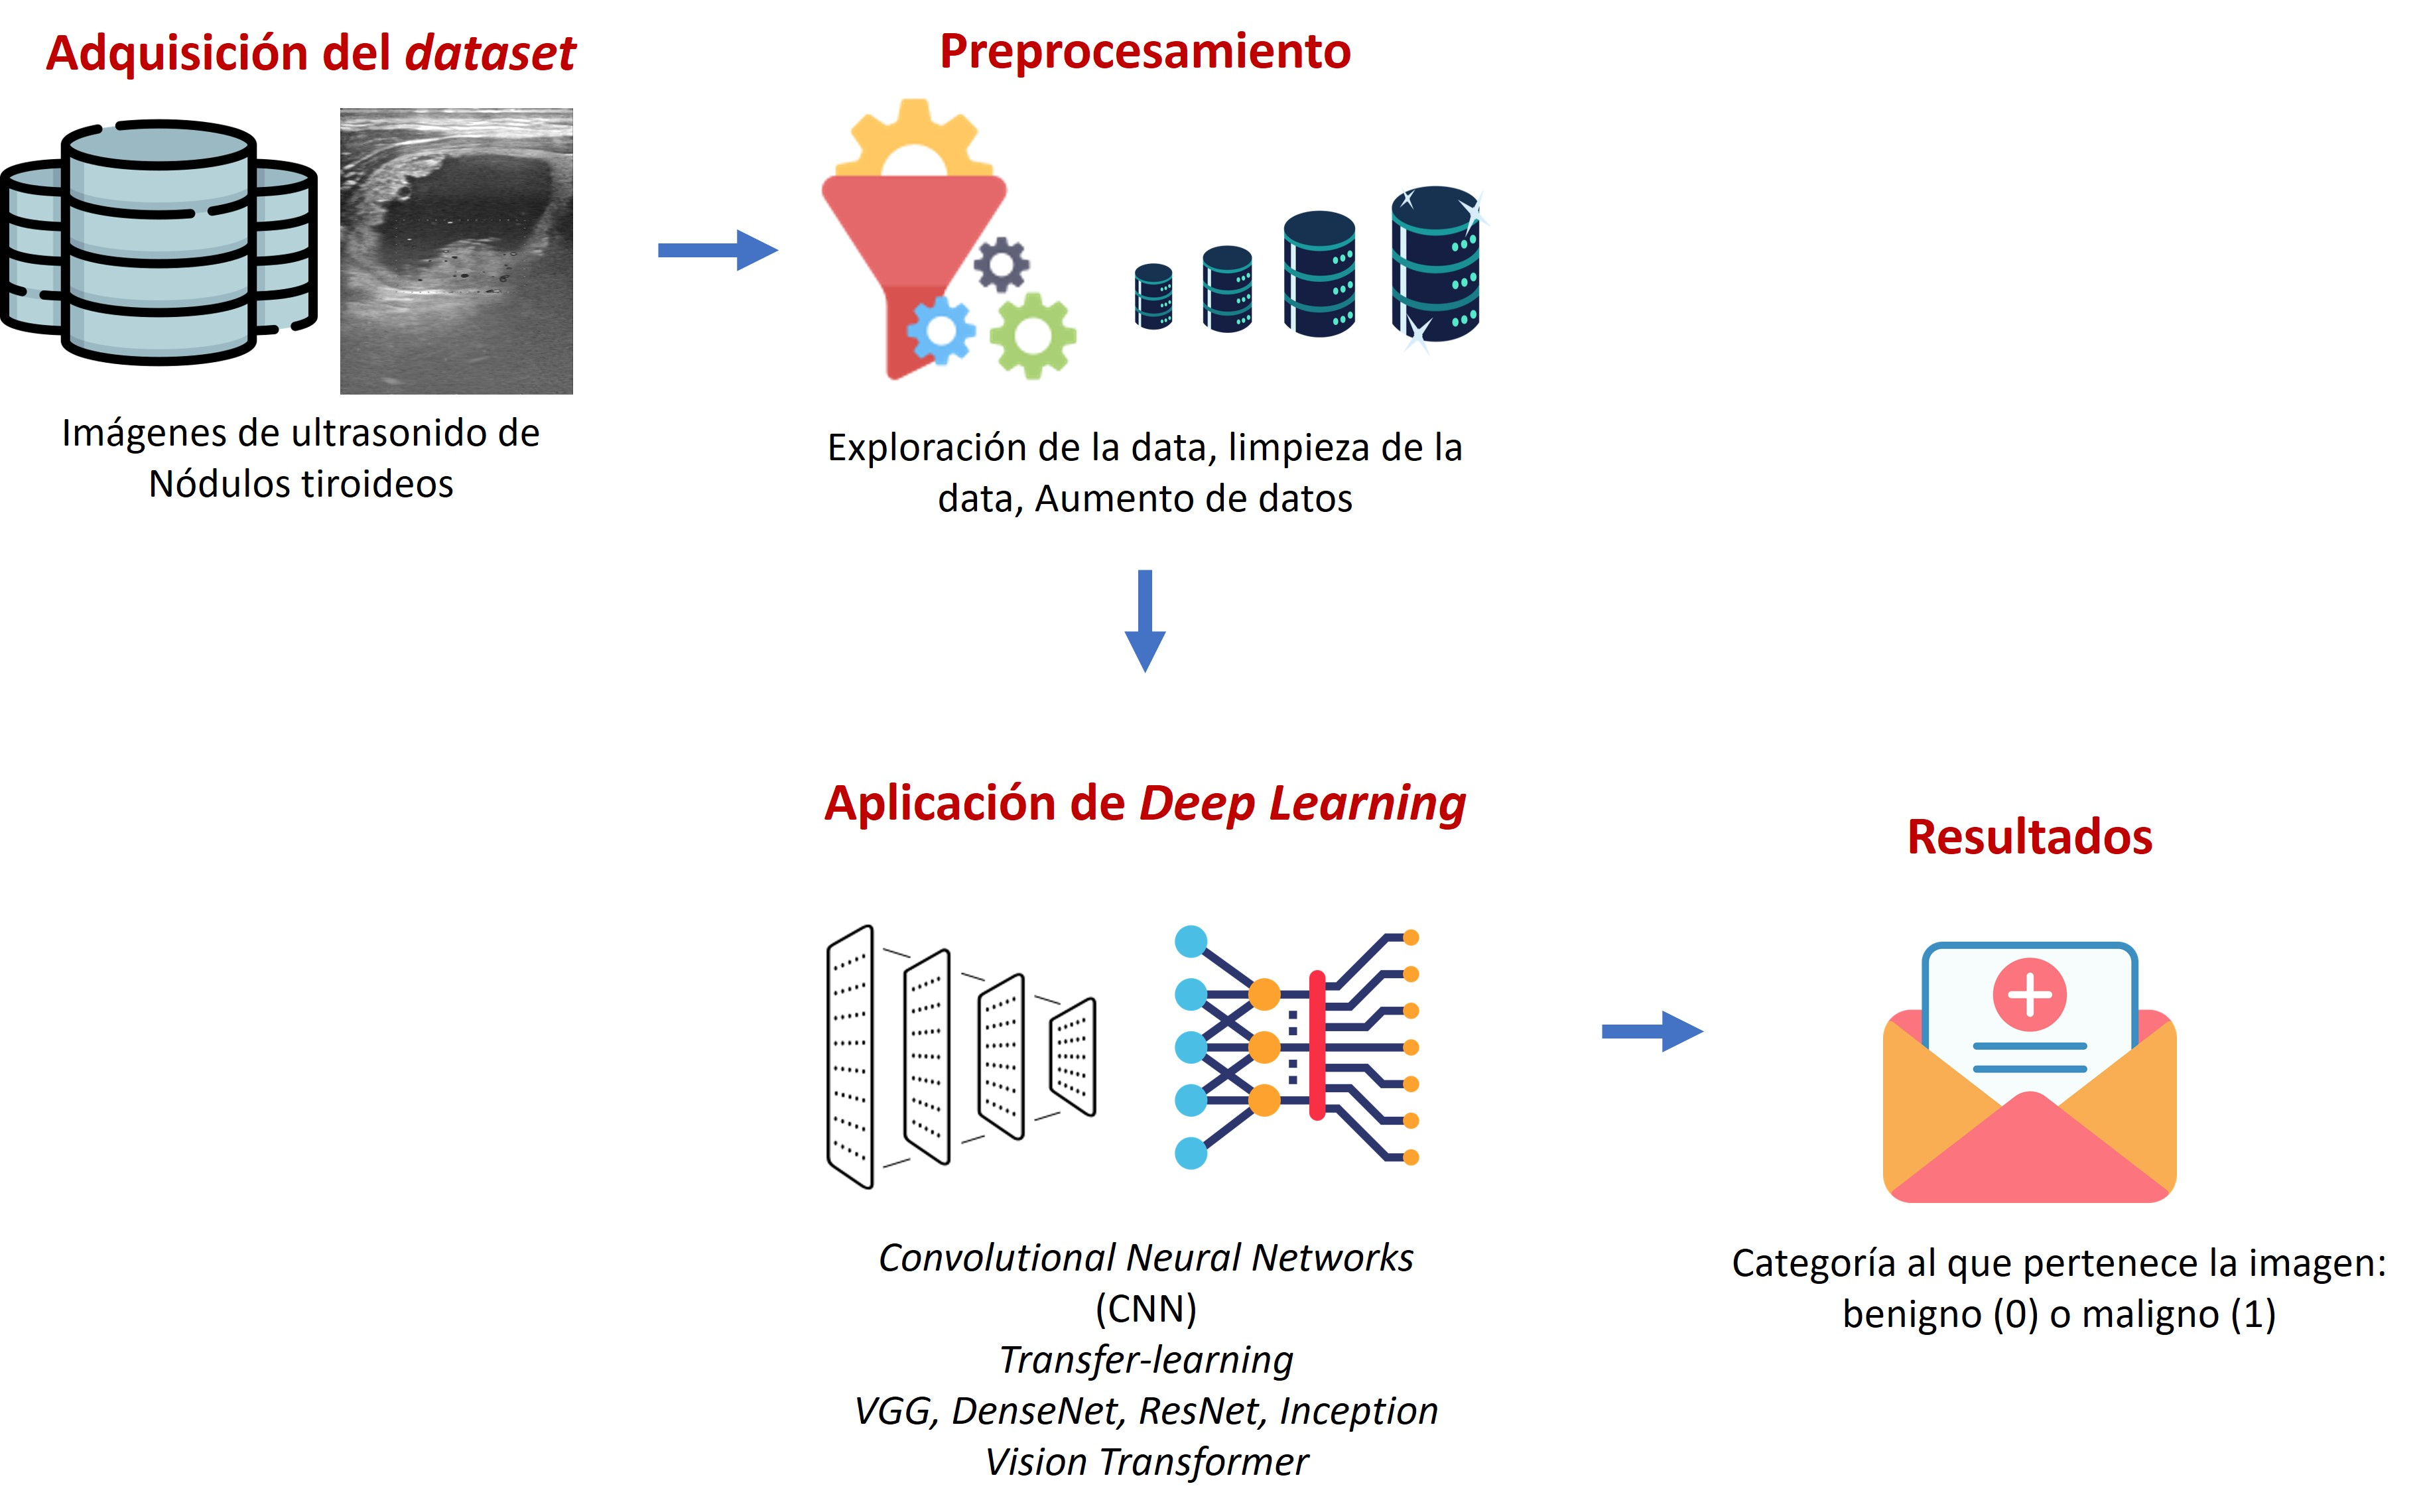
\includegraphics[width=1.00\textwidth]{3/figures/metod_classthy1.jpg}
		\caption[Metodología de implementación]{Metodología de implementación. \\
		Fuente: Elaboración propia.}
		\label{3:fig301}
	\end{center}
\end{figure}

La adquisición del conjunto de datos, es decir, imágenes de ultrasonido, consiste en la búsqueda y revisión de las bases de datos sobre imágenes de nódulos tiroideos, donde finalmente se seleccionará y descargará la de mayor utilidad. La base de datos debe cumplir con ciertos requerimientos para realizar un posterior entrenamiento del modelo que otorgue buenos resultados. Las imágenes deben ser debidamente etiquetadas según el carácter del nódulo al que representen, es decir, se debe indicar si cada una de las imágenes pertenece a la categoría benigno o maligno. Además, para evitar discrepancias entre calidad de imágenes en futuras evaluaciones, el conjunto de datos debe poseer imágenes de distintas instituciones de salud y de distintas calidades. Esto permitirá que el modelo entrenado no dependa de la una alta o baja calidad de las imágenes para realizar una correcta predicción. Finalmente, la cantidad de datos debe ser relativamente alta con el fin de aumentar la capacidad de generalización del modelo y evitar posibles sobreajustes o bajo rendimiento.  

En la etapa de preprocesamiento, se realizará en primera instancia una exploración del conjunto de datos con el fin de entender su composición y las características a mejorar; por ejemplo, un posible desbalanceo de clases o presencia de imágenes corruptas o sin etiquetar. Posteriormente, se realizará limpieza datos en caso de imágenes corruptas o de nula utilidad. Además, se usarán técnicas de aumento de datos o weigthing en la situación de desbalanceo de datos, con el fin de evitar una baja generalización y sobreajuste en la clase mayoritaria.  Finalmente, se aplicará escalado en las imágenes destinadas al entrenamiento del modelo con el objetivo de reducir la complejidad computacional y así obtener menor tiempo de ejecución.

Una vez se tenga la data ya preprocesada, este se usará como entrada para los modelos de Deep Learning. Principalmente, se planea usar algunos de los diversos tipos y arquitecturas de redes neuronales convolucionales (CNN), específicamente los más utilizados en este tipo de tareas como lo son VGG, RestNet, Inception y DenseNet, pues son ideales para la extracción de características de las imágenes, facilitando así el proceso final de clasificación. 

Cada uno de los modelos serán probados en parte de la data, específicamente en la data de prueba o test. De aquí se obtendrán las predicciones de los modelos clasificando las imágenes en benigno (0) o maligno (1).

\section{Metodología para la Medición de Resultados de la Implementación}

Los resultados obtenidos de la clasificación de los modelos previamente entrenados deberán ser evaluados para una correcta elección final. 

Antes de presentar las métricas a usar, es necesario conocer a la matriz de confusión y las partes que lo conforman, pues servirá como base para entenderlas. 

Según \cite{ws_izco2018bdcp} la matriz de confusión es una herramienta que permite ver de forma más clara el rendimiento de nuestro modelo.

\begin{figure}[H]
	\begin{center}
		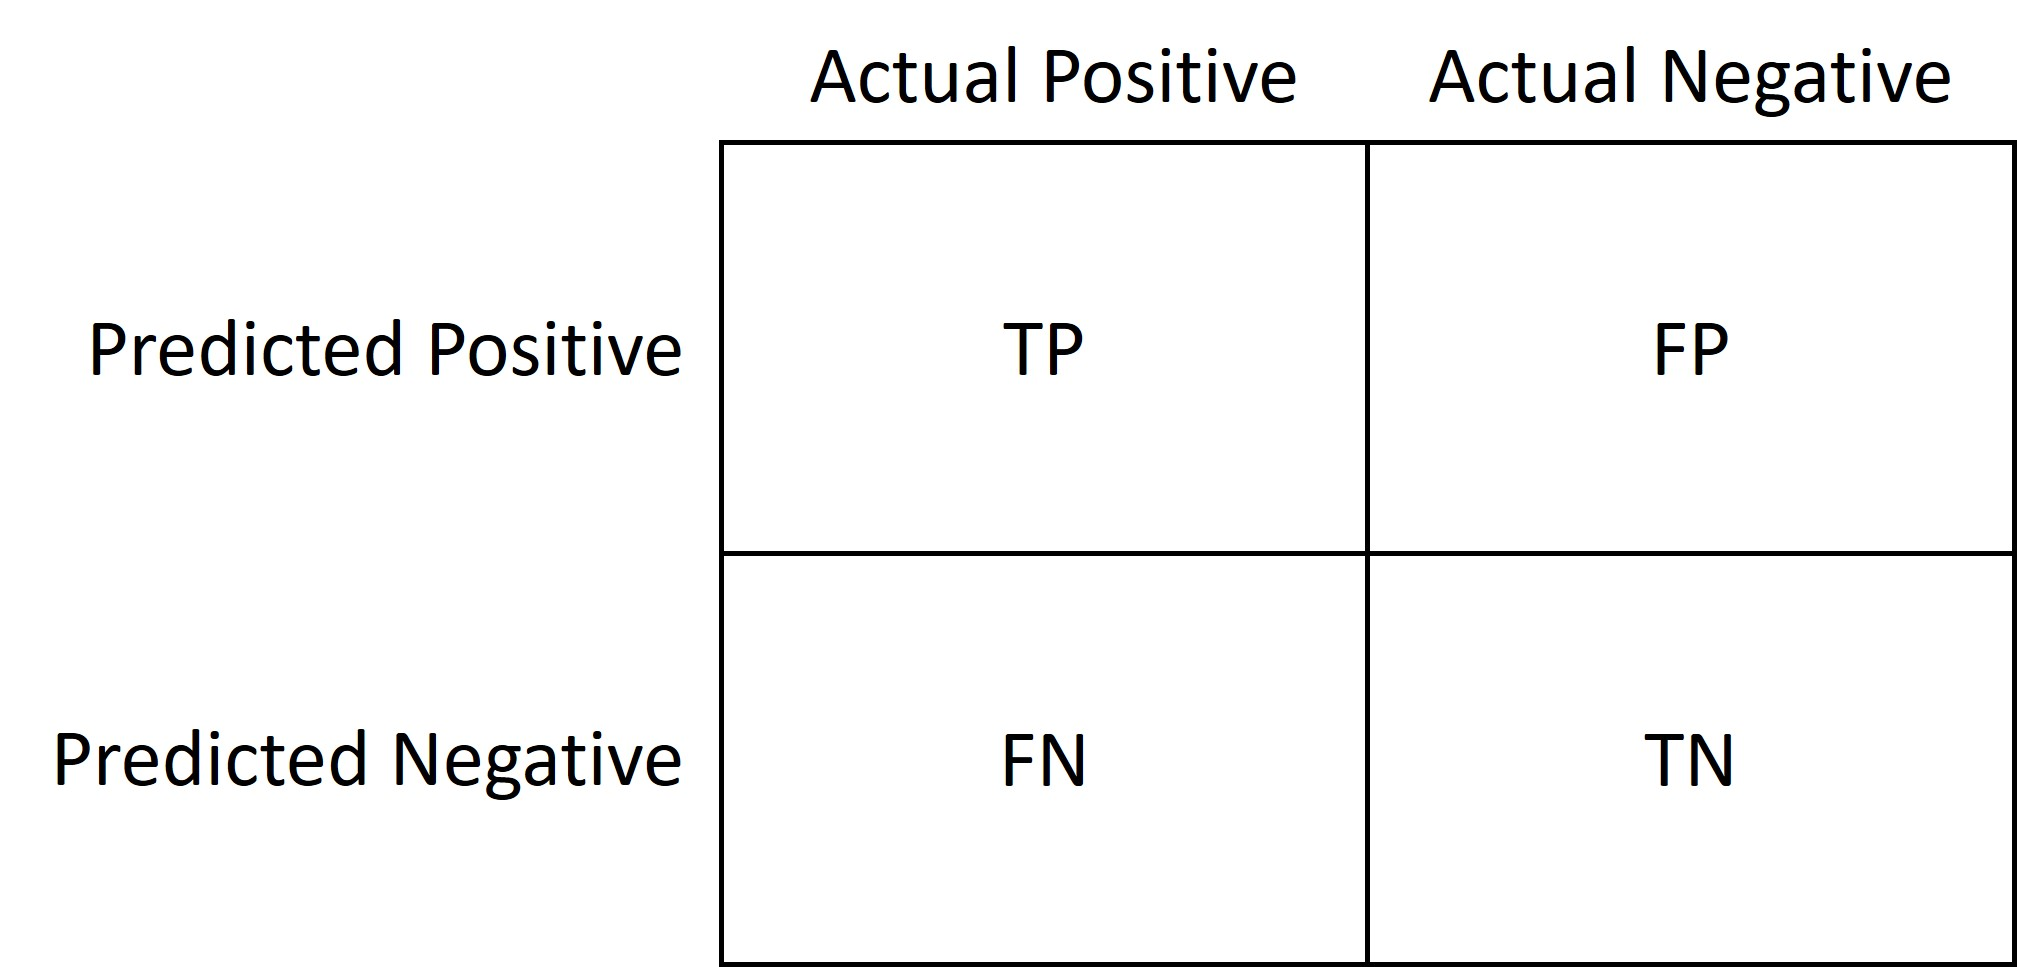
\includegraphics[width=0.75\textwidth]{3/figures/conf_matrix.jpg}
		\caption[Matriz de Confusión]{Matriz de Confusión. \\
		Fuente: Elaboración propia.}
		\label{3:fig302}
	\end{center}
\end{figure}

La matriz consta de cuatro partes importantes: TP, FP, FN y TN. Estos serán usados para presentar las fórmulas de las métricas más adelante. El primero (TP o true positive) se refiere a la cantidad de observaciones que se han predicho como positivos y que en verdad sí son positivos; por el contrario, FP (false positive) se refiere a aquellas predicciones dadas como positivos, pero en verdad son negativos. FN (false negative) es la cantidad de observaciones predichas como negativas; sin embargo, estas en realidad son positivas. Finalmente, TN (true negative) es la cantidad de observaciones predichas como negativas y que en realidad son también negativas.

A continuación, se presenta las métricas para medir el desempeño de la clasificación del modelo.

El accuracy representa aquella proporción del total de predicciones que se ha obtenido correctamente \parencite{ws_izco2018bdcp}. Este se calcula a través de la siguiente fórmula 1.

%\begin{equcaption}[!ht]
\begin{equation}\label{eq:accuracy}
\phantomsection
accuracy=\frac{TP+TN}{TP+TN+FP+FN}
\end{equation}
\myequations{Fórmula para calcular el accuracy}

El recall representa la proporción de solo los positivos reales predichos de manera acertada \parencite{ws_izco2018bdcp}. Se calcula con la siguiente fórmula.

%\begin{equcaption}[!ht]
\begin{equation}\label{eq:recall}
\phantomsection
recall=\frac{TP}{TP+FN}
\end{equation}
\myequations{Fórmula para calcular el recall}

Precision representa aquella proporción de lo predicho positivamente que es positiva \parencite{ws_izco2018bdcp}. Se calcula con la fórmula a continuación.

%\begin{equcaption}[!ht]
\begin{equation}\label{eq:precision}
\phantomsection
precision=\frac{TP}{TP+FP}
\end{equation}
\myequations{Fórmula para calcular el precision}

\begin{landscape}
	\section{Cronograma de actividades y presupuesto}
	Se propuso un cronograma para la investigación. Este conforma desde el inicio hasta ser terminada con la sustentación final planeada para mediados del año 2024.

	\begin{figure}[!ht]
		\begin{center}
			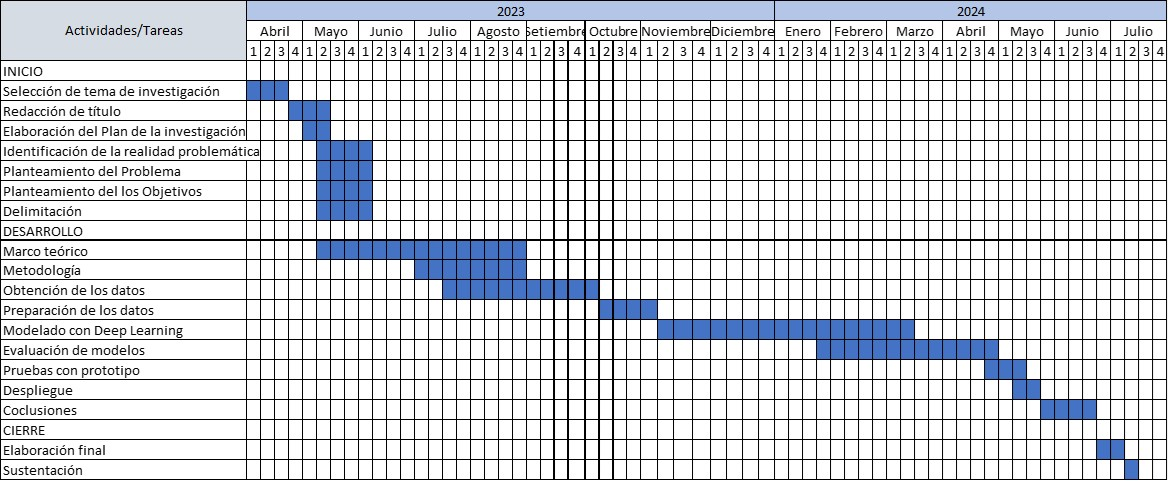
\includegraphics[width=1.50\textwidth]{3/figures/cronograma_tesis_thyr.jpg}
			\caption[Cronograma de actividades]{Cronograma de actividades.\\
				Fuente: Elaboración propia.}
			\label{3:fig303}
		\end{center}
	\end{figure}
	
\end{landscape}

Además, se determinó el presupuesto necesario para la elaboración completa de la investigación.

\begin{table}[H]
	\caption[Presupuesto]{Presupuesto.}
	\label{3:table1}
	\centering
	\small
	\begin{tabular}{llll}
		\specialrule{.1em}{.05em}{.05em}
		{Grupo} & {Item} & {Costo (soles)} & {Subtotal} \\
		\specialrule{.1em}{.05em}{.05em}
		\multirow{2}{3cm}{Recursos materiales} & {Laptop} & {S/ 6,500.00} & {} \\
		{} & {Materiales de escritorio} & {S/ 100.00} & {6,600.00} \\
		\cline{1-4}
		\multirow{2}{3cm}{Software y trámites} & {Reserva de tema} & {S/ 2,700.00} & {} \\
		{} & {Derecho de inscripción} & {S/ 800.00} & {} \\
		{} & {Derecho de sustentación} & {S/ 1,500.00} & {} \\
		{} & {Software} & {S/ 50.00} & {} \\
		{} & {Renta de servidor en la nube} & {S/ 224.15} & {S/ 5,274.15} \\
		\cline{1-4}
		\multirow{2}{3cm}{Extras} & {Consultorías} & {S/ 100.00} & {} \\
		{} & {Movilidad} & {S/ 200.00} & {S/ 300.00} \\
		\specialrule{.1em}{.05em}{.05em} 
		{} & {Total} & {} & {S/ 12,174.15} \\
		\specialrule{.1em}{.05em}{.05em}
	\end{tabular}
	\begin{flushleft}	
		\small Fuente: Elaboración propia.
	\end{flushleft}
\end{table}



